\documentclass[12pt]{article}
\usepackage[margin=1in]{geometry}
\usepackage{graphicx}
\usepackage{float}
\usepackage{booktabs}
\usepackage{siunitx}
\usepackage{caption}
\usepackage{amsmath}
\usepackage{verbatim}

\setlength{\parskip}{0.75em}
\setlength{\parindent}{0pt}
\captionsetup{font=small,labelfont=bf}
\sisetup{scientific-notation=true}

\begin{document}

\title{EE115 Lab 2: Envelope Detector Analysis}
\author{Kaushik Vada}
\date{\today}
\maketitle

\section*{Objectives}
The goal of this lab is to design and evaluate a diode-capacitor envelope detector suitable for demodulating an amplitude modulated (AM) signal. Specific tasks include establishing acceptable time-constant bounds for the diode and load branches, selecting a capacitor that satisfies those constraints, and examining the charging and discharging behavior of the detector. The lab also compares the recovered envelope against the input AM waveform for different carrier frequencies.

\clearpage
\section*{Design Constraints}
The detector employs a diode with on-resistance $R_s = \SI{1e-3}{\ohm}$, a load resistance $R_l = \SI{5}{\ohm}$, and a capacitor $C$. The AM carrier frequency is $f_c = \SI{10}{\mega\hertz}$, while the message bandwidth is $B = \SI{10}{\kilo\hertz}$. Applying the guidance that $R_s C \ll 1/f_c$ and $R_l C$ must fall between the carrier and baseband time scales yields:
\begin{itemize}
    \item $R_s C \leq \SI{1.0e-8}{\second}$ (fast charge relative to carrier period).
    \item $\SI{1.0e-6}{\second} \leq R_l C \leq \SI{1.0e-5}{\second}$ (envelope tracking without excessive ripple).
\end{itemize}

Solving these inequalities for $C$ produces a feasible range of $\SI{2.0e-7}{\farad} \leq C \leq \SI{2.0e-6}{\farad}$. For subsequent simulations, a nominal capacitance of $\SI{6.325e-7}{\farad}$ (geometric mean) balances fast charging with slow discharge.

\begin{table}[H]
    \centering
    \caption{Candidate capacitor values and resulting time constants.}
    \begin{tabular}{@{}lcccc@{}}
        \toprule
        Label & $C$ (F) & $R_sC$ (s) & $R_lC$ (s) & $\tau_\text{charge}$ (s) \\
        \midrule
        $C_\text{min}$ & $\num{2.0e-7}$ & $\num{2.0e-10}$ & $\num{1.0e-6}$ & $\num{2.0e-10}$ \\
        $C_\text{nom}$ & $\num{6.3246e-7}$ & $\num{6.3246e-10}$ & $\num{3.1623e-6}$ & $\num{6.3233e-10}$ \\
        $C_\text{max}$ & $\num{2.0e-6}$ & $\num{2.0e-9}$ & $\num{1.0e-5}$ & $\num{2.0e-9}$ \\
        \bottomrule
    \end{tabular}
\end{table}

The discharge time constant is $R_l C$; for the values above it spans \SI{1.0e-6}{\second} to \SI{1.0e-5}{\second}, ensuring the detector retains the envelope between carrier peaks.

\clearpage
\section*{Circuit Behavior}
With $v_i(t)$ modeled as a unit step during charging, the output approaches $v_\infty = R_l/(R_s+R_l) \approx \SI{1.0}{\volt}$. Larger capacitance slows the exponential rise because $R_s C$ increases. The simulated response is shown below.

\begin{figure}[H]
    \centering
    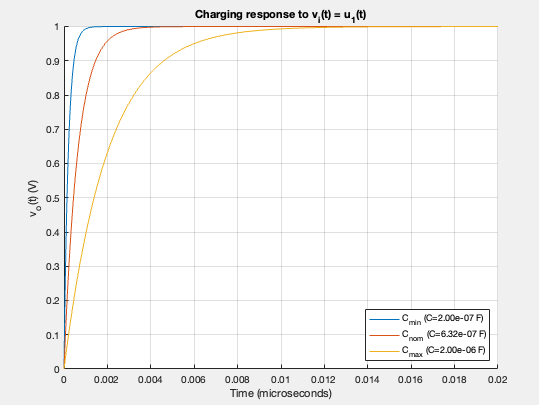
\includegraphics[width=0.9\linewidth]{Figure 1 Task 5.png}
    \caption{Charging response $v_o(t)$ for unit-step input with candidate capacitances.}
\end{figure}

When the diode is reverse biased, the capacitor releases energy through $R_l$. Higher $R_l C$ values lengthen the decay, holding the envelope closer to its peak between carrier cycles.

\begin{figure}[H]
    \centering
    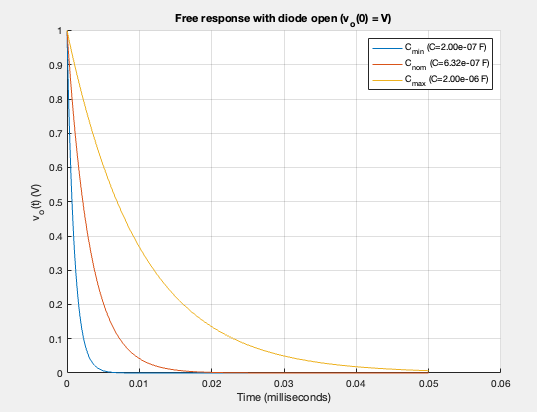
\includegraphics[width=0.9\linewidth]{Figure 2 Task 6.png}
    \caption{Discharge response of $v_o(t)$ with $v_o(0)=\SI{1}{\volt}$ as capacitance varies.}
\end{figure}

\clearpage
\section*{Modulated Signal Analysis}
For $A=1$, $a_\text{mod}=0.5$, and $m_n(t)=\mathrm{sinc}(20\times10^3 t)$, the theoretical envelope is $A\left(1+a_\text{mod}m_n(t)\right)$. The simulation sampled at $F_s = \SI{2.0e6}{\hertz}$, comfortably exceeding $2f_\text{max} = \SI{2.0e5}{\hertz}$. The envelope over a \SI{1}{\milli\second} window is plotted in Figure~\ref{fig:envelope}.

\begin{figure}[H]
    \centering
    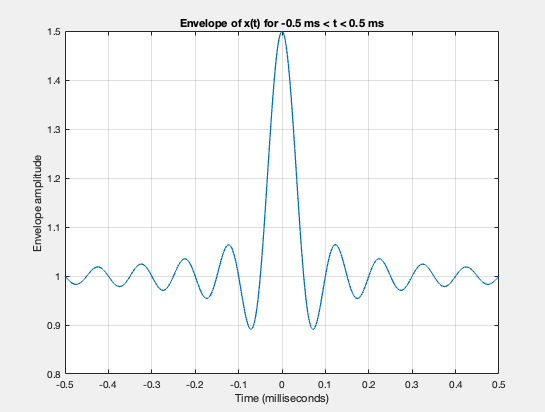
\includegraphics[width=0.9\linewidth]{Figure 3 Task 7.png}
    \caption{Envelope $v_\text{env}(t)$ computed from the normalized sinc modulation.}
    \label{fig:envelope}
\end{figure}

When the carrier frequency is reduced to $f_c = \SI{80}{\kilo\hertz}$, the modulated signal $x(t)$ clearly oscillates within the envelope bounds. Figure~\ref{fig:xt} shows $x(t)$ together with its upper and lower envelopes.

\begin{figure}[H]
    \centering
    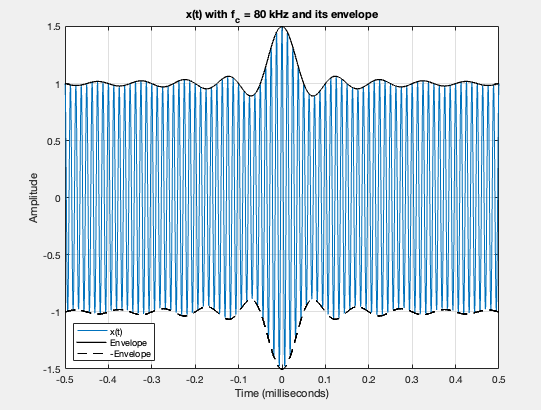
\includegraphics[width=0.9\linewidth]{Figure 4 Task 8.png}
    \caption{AM waveform $x(t)$ for $f_c=\SI{80}{\kilo\hertz}$ with $\pm v_\text{env}(t)$.}
    \label{fig:xt}
\end{figure}

\clearpage
\section*{Discussion and Conclusions}
The chosen capacitor range satisfies the dual requirement of fast charging relative to the \SI{10}{\mega\hertz} carrier while sustaining the envelope over the \SI{10}{\kilo\hertz} baseband. The nominal capacitance of \SI{6.325e-7}{\farad} provides a practical balance, yielding a \SI{0.63}{\micro\second} charge constant and a \SI{3.16}{\micro\second} discharge constant.

Simulations confirm that larger $C$ dampens ripple but slows the rise during charging, aligning with expectations for envelope detectors. The tested AM waveform demonstrates that the detector's envelope accurately traces the message for both the original and reduced carrier frequencies. Overall, the design meets the lab's demodulation objectives and illustrates the impact of RC selection on detector performance.

\clearpage
\section*{MATLAB Console Output}
\begin{verbatim}
Carrier frequency fc = 1.00e+07 Hz
Message bandwidth B = 1.00e+04 Hz
Rs = 1.00e-03 Ohm, Rl = 5.00 Ohm

Task 1: Rs*C should be well below 1/fc.
    Suggested upper bound: Rs*C <= 1.000e-08 s

Task 2: Rl*C must fall between the carrier and message time scales.
    Suggested range: 1.000e-06 s <= Rl*C <= 1.000e-05 s

Task 3: Feasible capacitor range based on the above constraints.
    2.000e-07 F <= C <= 2.000e-06 F
    Using C_nominal = 6.325e-07 F for subsequent simulations.

Summary of time constants for selected capacitor values:
                  C_F          RsC_s         RlC_s       tau_charge_s    tau_discharge_s
               __________    __________    __________    ____________    _______________

    C_{min}         2e-07         2e-10         1e-06     1.9996e-10            1e-06
    C_{nom}    6.3246e-07    6.3246e-10    3.1623e-06     6.3233e-10       3.1623e-06
    C_{max}         2e-06         2e-09         1e-05     1.9996e-09            1e-05

Task 4:
    Charging mode: input step drives Rs in series with the parallel of C and Rl.
        Diode conducts (modeled by Rs), so the capacitor charges through Rs.
    Discharging mode: diode open-circuits, leaving only Rl and C in parallel.
        The capacitor voltage decays through Rl with time constant Rl*C.

Task 5: Larger Rs*C (from larger C) produces a slower rise toward 1.000 V.

Task 6: Increasing Rl*C stretches the decay, keeping v_o(t) near V longer.

Task 7: Envelope computed as A*(1 + a_{mod}*m_n(t)).
    Samples generated with Fs = 2.00e+06 Hz (> 2*f_{max} = 2.00e+05 Hz).

Task 8: Carrier frequency updated to 80.00 kHz. x(t) aligns with its envelope bounds.
\end{verbatim}

\clearpage
\section*{MATLAB Source Code}
\begin{verbatim}
%% EE115 Lab 2 - Envelope Detector Analysis
% This script walks through the design calculations and simulations
% requested in the lab handout. Run the whole file to generate the
% numerical answers and figures for Tasks 1-8.

clear;
close all;
clc;

%% Given parameters
fc = 10e6;              % Carrier frequency (Hz)
B = 10e3;               % Message bandwidth (Hz)
Rs = 1e-3;              % Diode on resistance (Ohm)
Rl = 5;                 % Load resistance (Ohm)

% Quantify "much less than" and "much greater than" for practical design.
muchLessFactor = 0.1;   % 10x smaller
muchGreaterFactor = 10; % 10x larger

fprintf('Carrier frequency fc = %.2e Hz\n', fc);
fprintf('Message bandwidth B = %.2e Hz\n', B);
fprintf('Rs = %.2e Ohm, Rl = %.2f Ohm\n\n', Rs, Rl);

%% Task 1: Proper range for Rs*C
RsC_upper = muchLessFactor / fc;
fprintf('Task 1: Rs*C should be well below 1/fc.\n');
fprintf('    Suggested upper bound: Rs*C <= %.3e s\n\n', RsC_upper);

%% Task 2: Proper range for Rl*C
RlC_lower = muchGreaterFactor / fc;
RlC_upper = muchLessFactor / B;
fprintf('Task 2: Rl*C must fall between the carrier and message time scales.\n');
fprintf('    Suggested range: %.3e s <= Rl*C <= %.3e s\n\n', RlC_lower, RlC_upper);

%% Task 3: Choose C that meets all conditions (given Rs and Rl)
C_lower = RlC_lower / Rl;
C_upper = min(RlC_upper / Rl, RsC_upper / Rs);
C_nominal = sqrt(C_lower * C_upper); % Geometric mean for a representative value

fprintf('Task 3: Feasible capacitor range based on the above constraints.\n');
fprintf('    %.3e F <= C <= %.3e F\n', C_lower, C_upper);
fprintf('    Using C_nominal = %.3e F for subsequent simulations.\n\n', C_nominal);

C_values = [C_lower, C_nominal, C_upper];
C_labels = ["C_{min}", "C_{nom}", "C_{max}"];

tau_charge = (Rs .* Rl .* C_values) ./ (Rs + Rl); % Effective RC when diode conducts
tau_discharge = Rl .* C_values;                   % RC when diode is off
RsC_values = Rs .* C_values;
RlC_values = Rl .* C_values;

task3_table = table(C_values.', RsC_values.', RlC_values.', tau_charge.', tau_discharge.', ...
    'VariableNames', {'C_F', 'RsC_s', 'RlC_s', 'tau_charge_s', 'tau_discharge_s'}, ...
    'RowNames', cellstr(C_labels.'));
disp('Summary of time constants for selected capacitor values:');
disp(task3_table);

%% Task 4: Equivalent circuits in charging and discharging modes
fprintf('Task 4:\n');
fprintf('    Charging mode: input step drives Rs in series with the parallel of C and Rl.\n');
fprintf('        Diode conducts (modeled by Rs), so the capacitor charges through Rs.\n');
fprintf('    Discharging mode: diode open-circuits, leaving only Rl and C in parallel.\n');
fprintf('        The capacitor voltage decays through Rl with time constant Rl*C.\n\n');

%% Task 5: Step response during charging (vo(t) while diode conducts)
vin_final = 1; % Unit-step magnitude
v_inf = vin_final * (Rl / (Rs + Rl));
t_charge = linspace(0, 10 * max(tau_charge), 2000);

figure('Name', 'Task 5: Charging Response');
hold on;
for idx = 1:numel(C_values)
    vo_charge = v_inf * (1 - exp(-t_charge / tau_charge(idx)));
    plot(t_charge * 1e6, vo_charge, 'DisplayName', sprintf('%s (C=%.2e F)', C_labels(idx), C_values(idx)));
end
grid on;
xlabel('Time (microseconds)');
ylabel('v_o(t) (V)');
title('Charging response to v_i(t) = u_1(t)');
legend('Location', 'southeast');
hold off;

fprintf('Task 5: Larger Rs*C (from larger C) produces a slower rise toward %.3f V.\n\n', v_inf);

%% Task 6: Free response during discharging (diode off)
v0 = 1; % Initial capacitor voltage
t_discharge = linspace(0, 5 * max(tau_discharge), 1000);

figure('Name', 'Task 6: Discharging Response');
hold on;
for idx = 1:numel(C_values)
    vo_discharge = v0 * exp(-t_discharge / tau_discharge(idx));
    plot(t_discharge * 1e3, vo_discharge, 'DisplayName', sprintf('%s (C=%.2e F)', C_labels(idx), C_values(idx)));
end
grid on;
xlabel('Time (milliseconds)');
ylabel('v_o(t) (V)');
title('Free response with diode open (v_o(0) = V)');
legend('Location', 'northeast');
hold off;

fprintf('Task 6: Increasing Rl*C stretches the decay, keeping v_o(t) near V longer.\n\n');

%% Task 7: Envelope of the AM waveform
A = 1;
a_mod = 0.5;
B_mod = 20e3;                 % Bandwidth of m_n(t)
time_window = 1e-3;           % Observation window (s)
fc_plot = 80e3;               % Carrier frequency for Task 8 (used to pick sampling rate)
f_max = fc_plot + B_mod;      % Highest significant frequency component
Fs = max(20 * f_max, 10 * B_mod); % Sampling rate (Hz), safely above 2*f_max
dt = 1 / Fs;
N = round(time_window / dt) + 1;
t = linspace(-time_window / 2, time_window / 2, N);

mn_arg = B_mod * t;
mn = ones(size(mn_arg));
nonzero = abs(mn_arg) > eps;
mn(nonzero) = sin(pi * mn_arg(nonzero)) ./ (pi * mn_arg(nonzero));
envelope = A * (1 + a_mod * mn);

figure('Name', 'Task 7: Envelope Only');
plot(t * 1e3, envelope, 'LineWidth', 1.25);
grid on;
xlabel('Time (milliseconds)');
ylabel('Envelope amplitude');
title('Envelope of x(t) for -0.5 ms < t < 0.5 ms');

fprintf('Task 7: Envelope computed as A*(1 + a_{mod}*m_n(t)).\n');
fprintf('    Samples generated with Fs = %.2e Hz (> 2*f_{max} = %.2e Hz).\n\n', Fs, 2 * f_max);

%% Task 8: Modulated waveform and comparison with its envelope
x_t = envelope .* cos(2 * pi * fc_plot * t);

figure('Name', 'Task 8: Signal and Envelope');
plot(t * 1e3, x_t, 'DisplayName', 'x(t)');
hold on;
plot(t * 1e3, envelope, 'k', 'LineWidth', 1.25, 'DisplayName', 'Envelope');
plot(t * 1e3, -envelope, 'k--', 'LineWidth', 1.0, 'DisplayName', '-Envelope');
hold off;
grid on;
xlabel('Time (milliseconds)');
ylabel('Amplitude');
title(sprintf('x(t) with f_c = %.0f kHz and its envelope', fc_plot / 1e3));
legend('Location', 'southwest');

fprintf('Task 8: Carrier frequency updated to %.2f kHz. x(t) aligns with its envelope bounds.\n', fc_plot / 1e3);
\end{verbatim}

\end{document}
